\documentclass{article}
\usepackage[utf8]{inputenc}
\usepackage{kotex} % 한국어를 가능하도록 해주는 패키지 입니다. 
\usepackage[left=2.5cm,right=2.5cm,top=3cm,bottom=3cm,a4paper]{geometry} % 페이지 레이아웃 설정입니다. 
\usepackage{listings}  % 소스코드 작성에 필요한 패키지 입니다. 헤더파일이랑 비슷한 개념입니다. 
% 소스코드는 \begin{lstlisting} 이 사이에 써야됩니다. \end{lstlisting}
% 이건 주석입니다. 
% // 이건 개행입니다. 
% \indent 이건 들여쓰기입니다. 
% 논문 링크는 references.bib에서 수정한 후에 
% 이 파일로 돌아와서 해당 부분에 \citep[이름] 코드를 붙여야합니다. 
% 사진의 경우 import 후 30번째 줄을 참고하시면 됩니다. 

\title{Darknet YOLO API}
\author{이대경, 김한섭, 강일송 }
\date{2017학년도 2학기 오픈소스 Team Project}

\usepackage{natbib}
\usepackage{graphicx}

\begin{document}

\maketitle

\section{You Only Look Once}

\indent YOLO시스템은 최첨단 실시간 물체 감지 시스템이다.
기존의 탐지시스템은 Repurpose classifiers 혹은 Localizers를 사용하여 탐지를 수행하였습니다. 이 방법은 모델의 여러 위치에 격자 이미지를 적용하는 방식이며 격자 중 높은 일치도를 보인 물체를 탐지합니다. 하지만 YOLO는 하나의 신경망을 전체 이미지에 적용하는 완전히 다른 방식을 사용합니다. 이 신경망은 이미지를 여러 영역으로 분할하고 각 영역에 대한 바운딩 영역과 가중치로 사용될 일치 확률을 예측하여 줍니다.

\begin{figure}[h!]
\centering
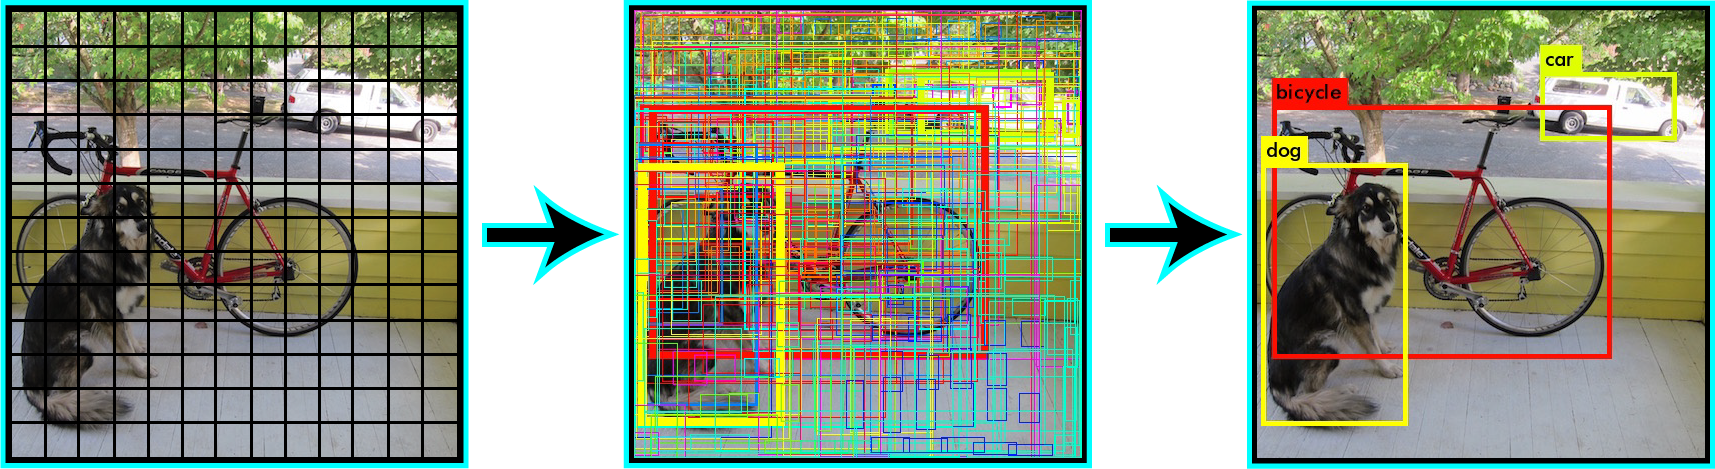
\includegraphics[scale=0.2]{model2.png}
\caption{탐지과정}
\label{fig:detect}
\end{figure}

YOLO 시스템은 분류 기반의 시스템에 비해 몇 가지 장점을 가지고 있다.
그 중 하나는 테스트 시간 동안 전체 이미지를 보고 예측된 정보를 이미지에 텍스트로 알려줍니다. 또한 수천개의 단일 이미지가 필요한 R-CNN 과는 달리 단일 네트워크만으로 평가하고 예측이 가능합니다. 이로 인해 R-CNN보다는 1000배 이상 빠르며 Fast R-CNN보다는 100배 빠릅니다. 전체 시스템에 대한 자세한 내용은 해당 논문\citep{YOLO9000} 을 참고하시기 바랍니다.


\section{탐지기법 실습}

\indent 사전 훈련 된 모델을 사용하여 YOLO 시스템으로 물체를 탐지 하는 방법을 설명합니다. 
Darknet을 아직 설치 하지 않았다면 먼저 설치 해야합니다. \\
이제부터 아래의 명령어를 실행하시기바랍니다.\\
\begin{lstlisting}.
git clone https://github.com/pjreddie/darknet
cd darknet 
make
\end{lstlisting}
실행 후 cfg/ 서브디렉토리에 YOLO에 대한 설정 파일이 존재합니다. 
\\사전 훈련된 가중치를 다운로드한 뒤
\begin{lstlisting}
wget https://pjreddie.com/media/files/yolo.wegith
\end{lstlisting}
다음을 실행하시기 바랍니다.
\begin{lstlisting}
/darknet detect cfg/yolo.cfg yolo.weights data/dog.jpg 
\end{lstlisting}
여기까지 실행하시면 다음과 같은 출력이 표시됩니다.\\
\begin{lstlisting}
   .layer filters size input output 
   0 conv 32 3 x 3 / 1 416 x 416 x 3 -> 416 x 416 x 32 
   1 max 2 x 2 / 2 416 x 416 x 32 -> 208 x 208 x 32 
   ....... 
   29 conv 425 1 x 1 / 1 13 x 13 x1024 -> 13 x 13 x 425 
   30 detection 
   Loading weights from yolo.weights...Done! 
   data/dog.jpg: Predicted in 0.016287 seconds. 
   car: 54% 
   bicycle: 51% 
   dog: 56% 
\end{lstlisting}

\begin{figure}[h!]
\centering
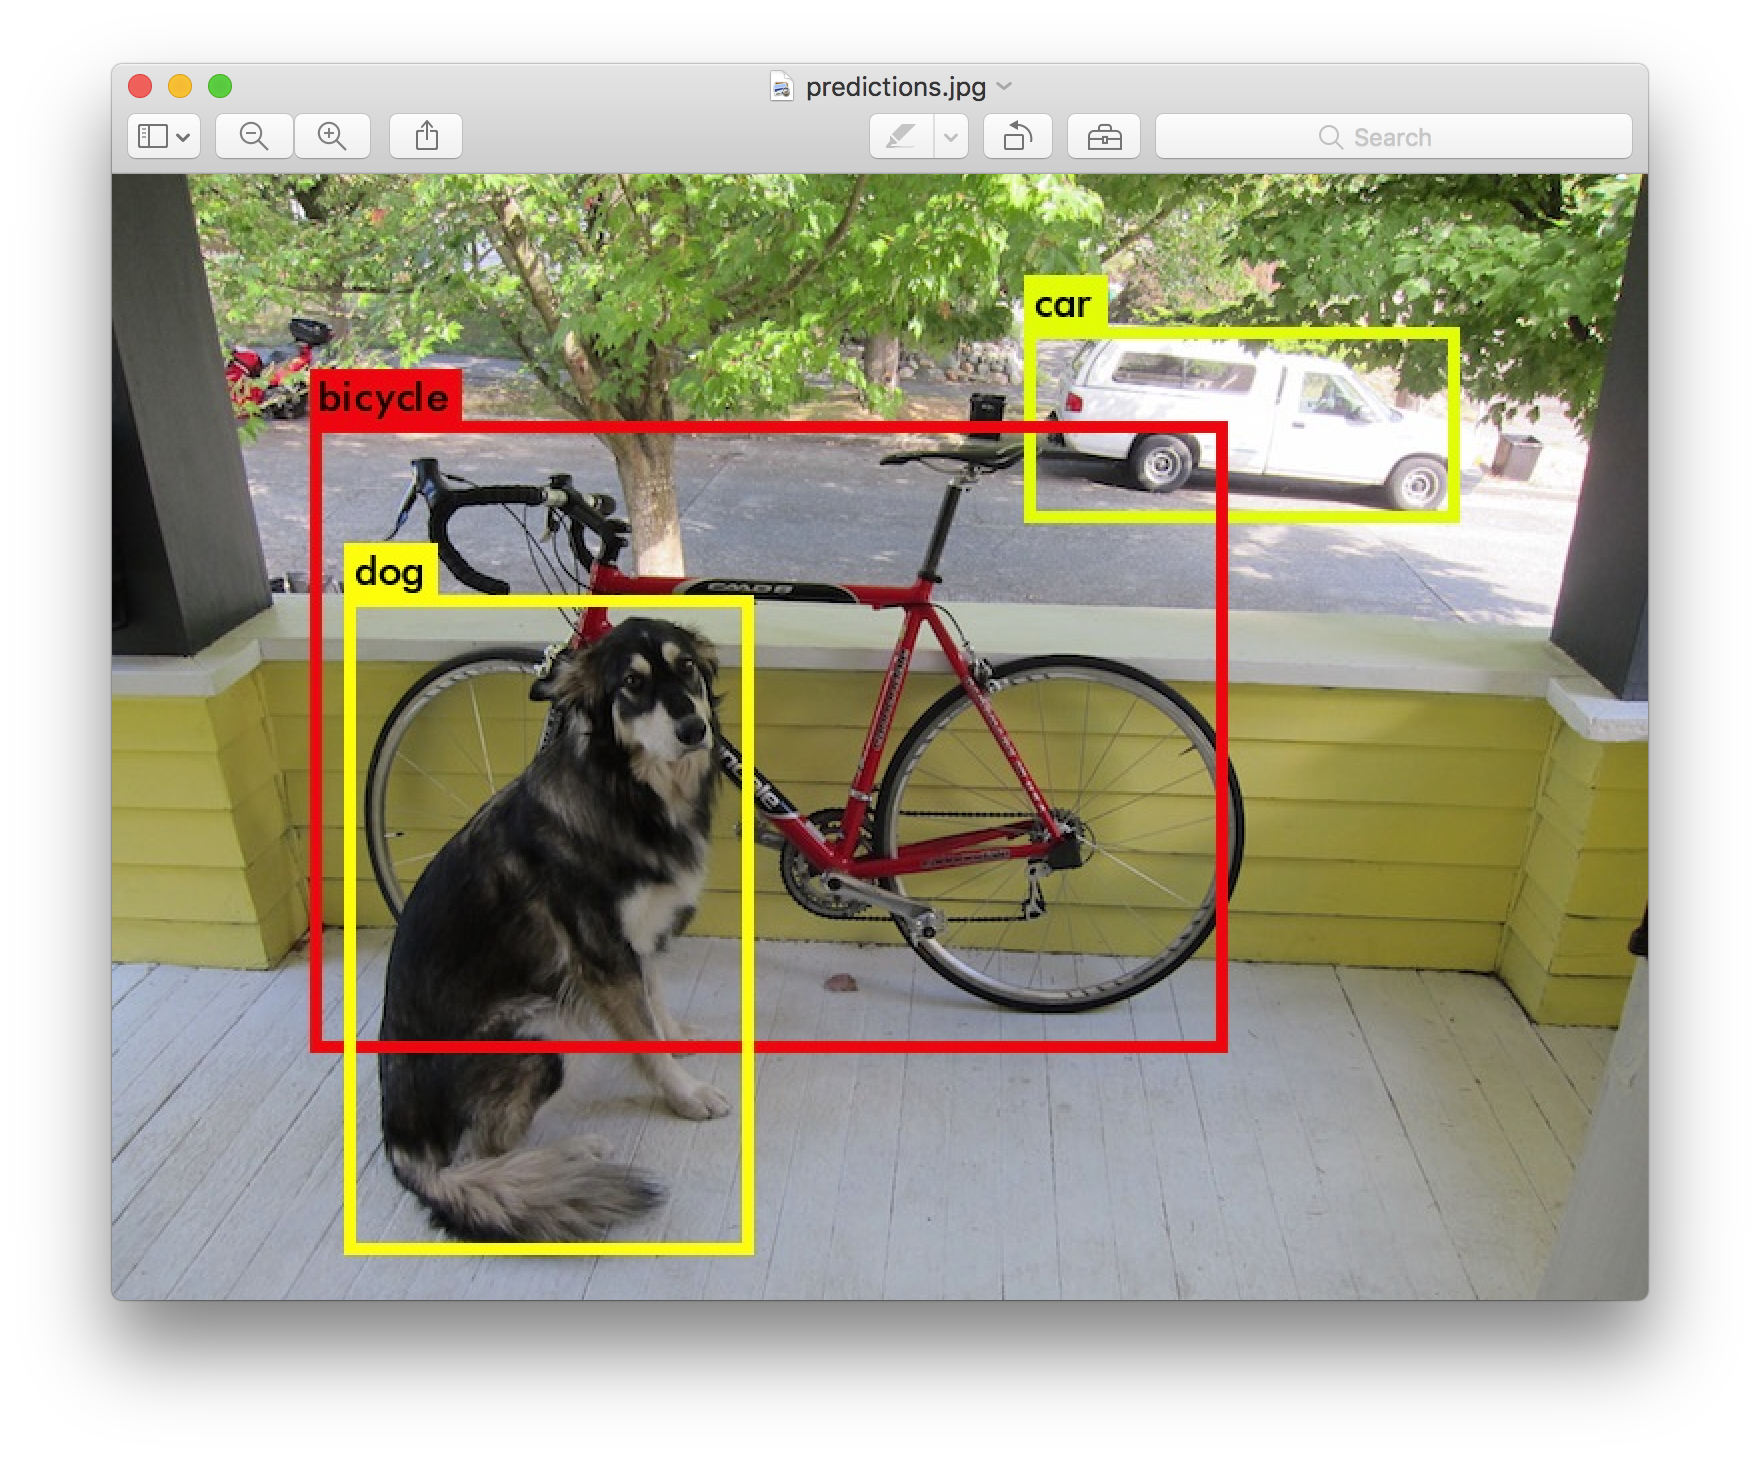
\includegraphics[scale=0.2]{ResultIMAGE.png}
\caption{탐지결과}
\label{fig:result}
\end{figure}

Darknet은 탐지한 객체와 일치도, 발견하는데 소요된 시간을 인쇄합니다.
해당 시스템은 Open CV를 이용해 컴파일하지 않았기 떄문에 탐지를 직접적으로 표시할 수 없습니다. 그렇기에 탐지된 내용을 predictions.png로 저장하고 사용자는 저장된 파일을 열어 탐지된 객체를 확인하는 방식을 사용하고 있습니다. 
해당 시스템은 CPU를 사용하기 때문에 하나의 이미지당 6초에서 12초가 소요됩니다. 
만약 GPU 환경을 사용한다면 더 빨라질 수 있습니다. 이해를 위한 몇 가지 예시 파일들을 포함시켜 놓았습니다. 확인해보시길 바랍니다. \\\\
1. data/eagle.jpg \\
2. data/dog.jpg \\
3. data/person.jpg \\
4. data/horses.jpg\\
\\
detect명령은 보다 일반적인 명령어 버전의 줄임말이며 다음 명령어와 동일합니다.

\begin{lstlisting}
./darknet detector test cfg/coco.data cfg/yolo.cfg yolo.weights data/dog.jpg 
\end{lstlisting}

하나의 이미지에서 탐지를 실행하는 시스템이지만 
웹캠에서 실행되는 것과 같은 다른 환경에서의 다른 작업을 수행 할 것인지를 아는 것이 유용하고
앞으로도 배우게 됩니다. 

\section{다중이미지 실습}
명령창에 이미지를 제공하는 대신 하나의 행에 여러 이미지를 시도해 볼 수 있으며 구성과 가중치가 완료되면 프롬포트가 표시됩니다.
\begin{lstlisting}
  ./darknet detect cfg/yolo.cfg yolo.weights 
  layer filters size input output 
  0 conv 32 3 x 3 / 1 416 x 416 x 3 -> 416 x 416 x 32 
  1 max 2 x 2 / 2 416 x 416 x 32 -> 208 x 208 x 32 
  ....... 
  29 conv 425 1 x 1 / 1 13 x 13 x1024 -> 13 x 13 x 425 
  30 detection 
  Loading weights from yolo.weights ...Done! 
  Enter Image Path: 
\end{lstlisting}
data/horses.jpg이미지의 경로를 입력하면 해당 이미지의 경계 영역을 예측하게 됩니다.
\begin{figure}[h!]
\centering
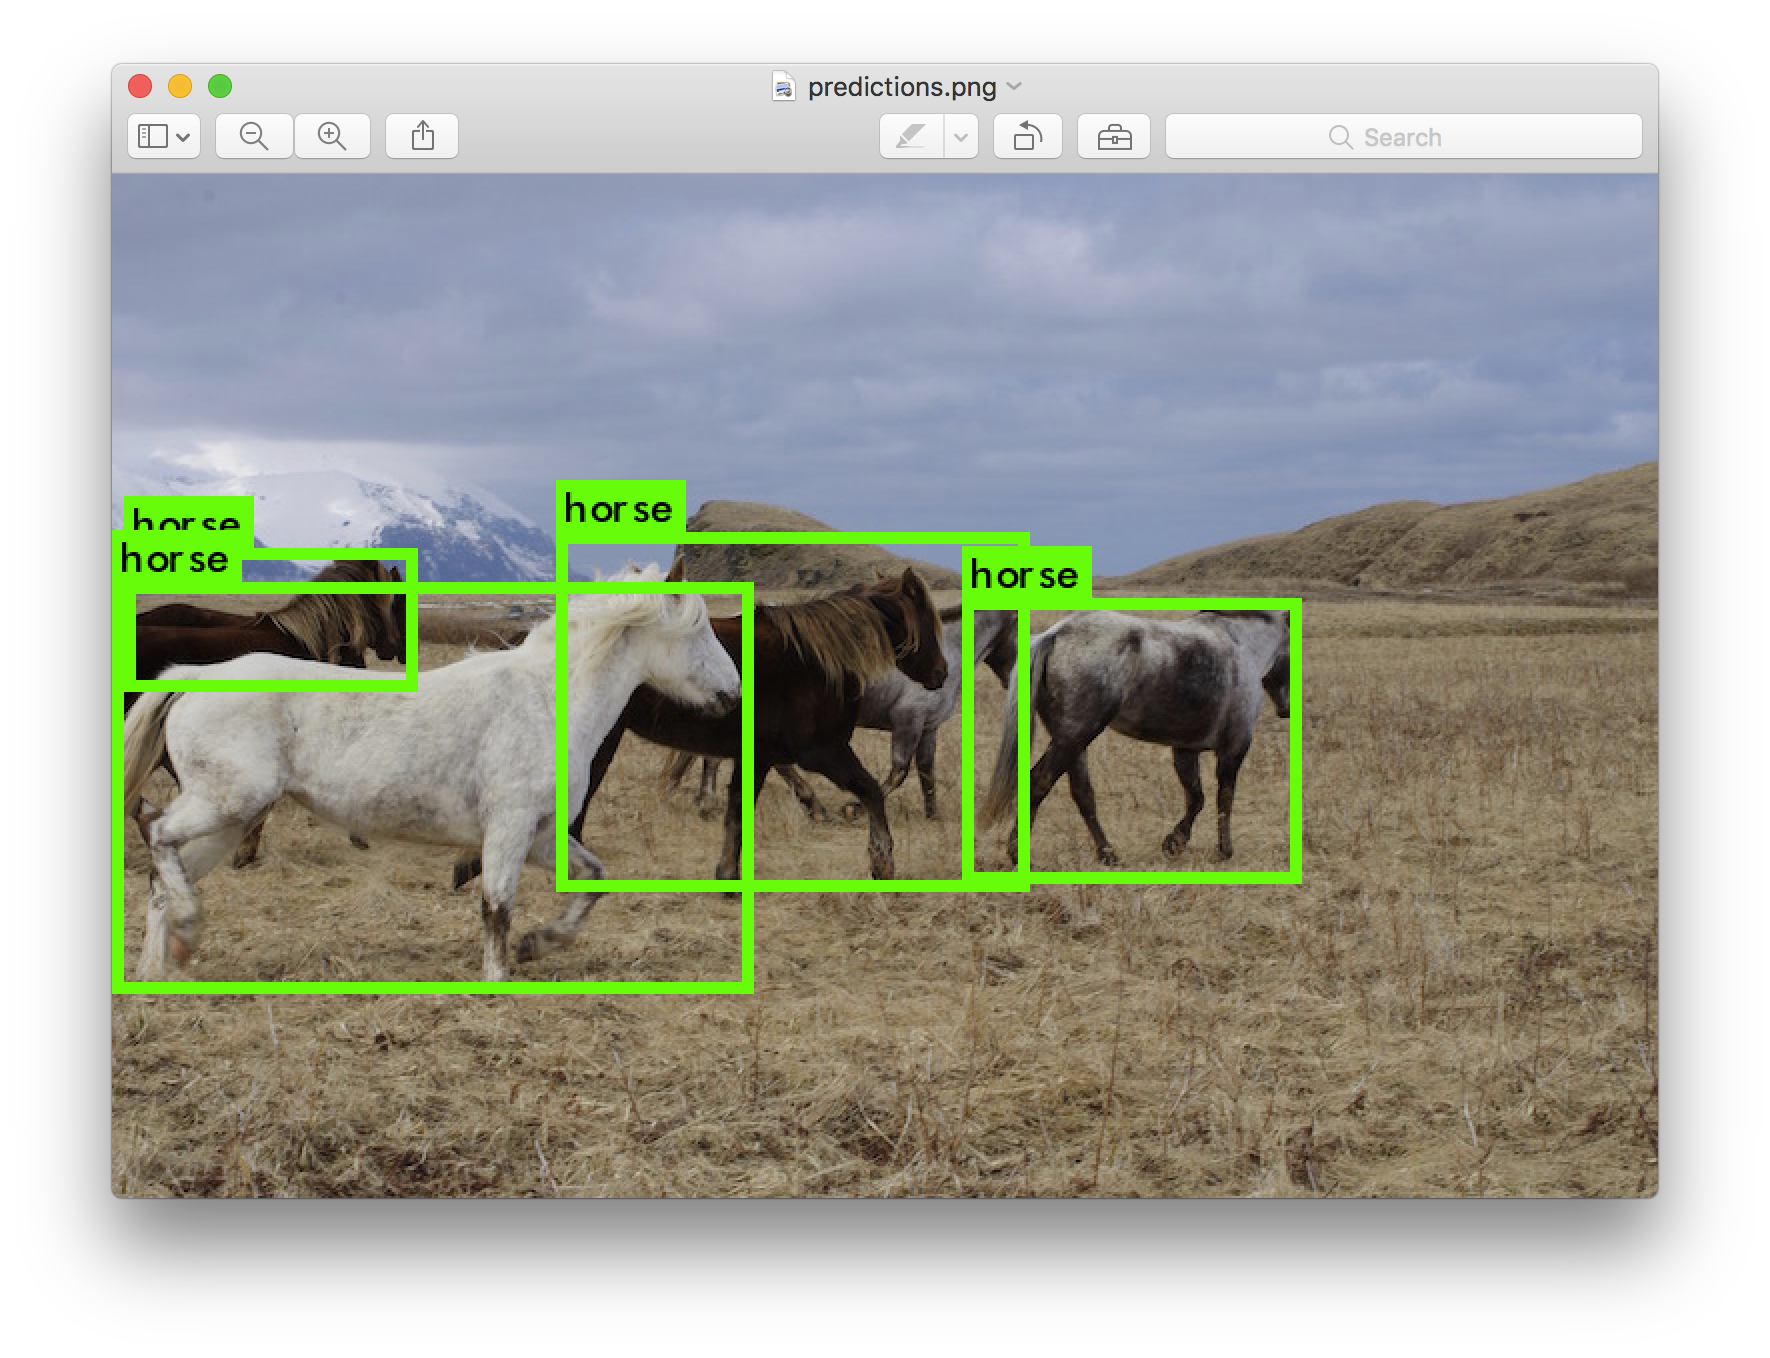
\includegraphics[scale=0.2]{horse.png}
\caption{탐지 결과}
\label{fig:horseresult}
\end{figure}
하나의 이미지가 완료되면 다른 이미지를 시도하귀 위해 더 많은 경로를 물어볼 것입니다.
Ctrl-C를 사용해 프로그램을 종료하시면 됩니다.
\section{탐색의 임계값 변경}
YOLO 시스템의 신뢰도는 기본값이 0.25이며 객체의 탐색 일치도가 0.25 이상인 객체만을 표시하여 사용자에게 보여줍니다.
이러한 임계값은 -thresh <val> 명령어 플래그를 이용하여 임계값을 변경 할 수 있습니다. 
아래의 예시는 탐색된 모든 객체를 표시하기 위하여 임계값을 0으로 설정한 것입니다. 예시 이미지를 참고하시기 바랍니다.
\begin{lstlisting}
 ./darknet detect cfg/yolo.cfg yolo.weights data/dog.jpg -thresh 0 
\end{lstlisting}
\begin{figure}[h!]
\centering
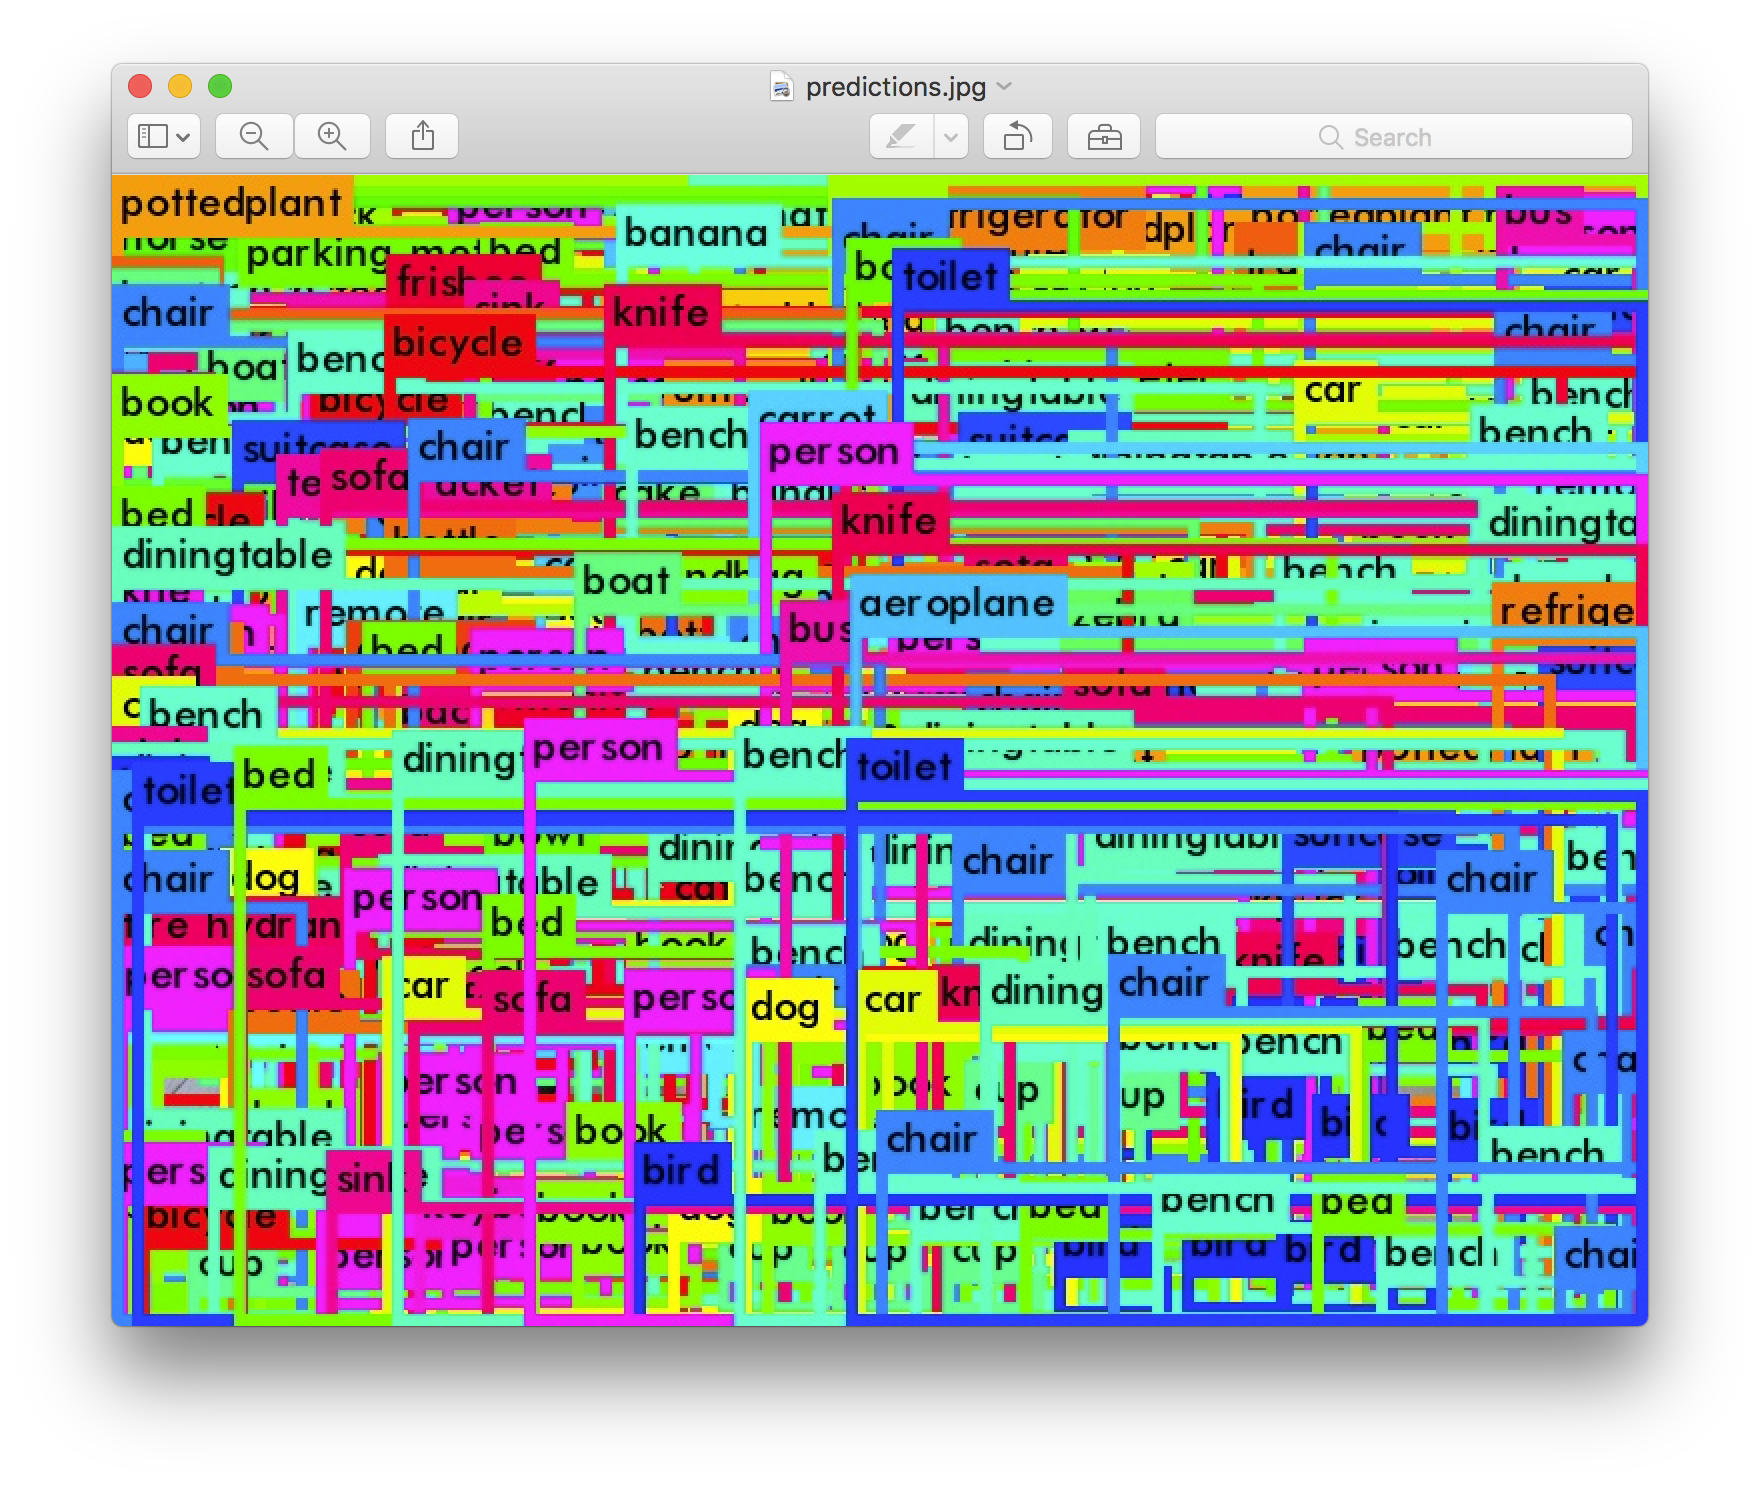
\includegraphics[scale=0.2]{eximage.png}
\caption{임계값 0 탐색결과 }
\label{fig:eximg}
\end{figure}


\bibliographystyle{plain}
\bibliography{references}
\end{document}
